\section{A common use-case}
\subsection{Retry my results}

\begin{frame}{A classic use case}
\centering{
\onslide<1->{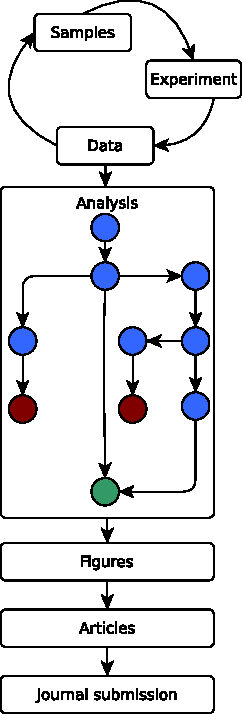
\includegraphics[width=0.17\textwidth]{schema_soumission_fair.pdf}}
\onslide<2->{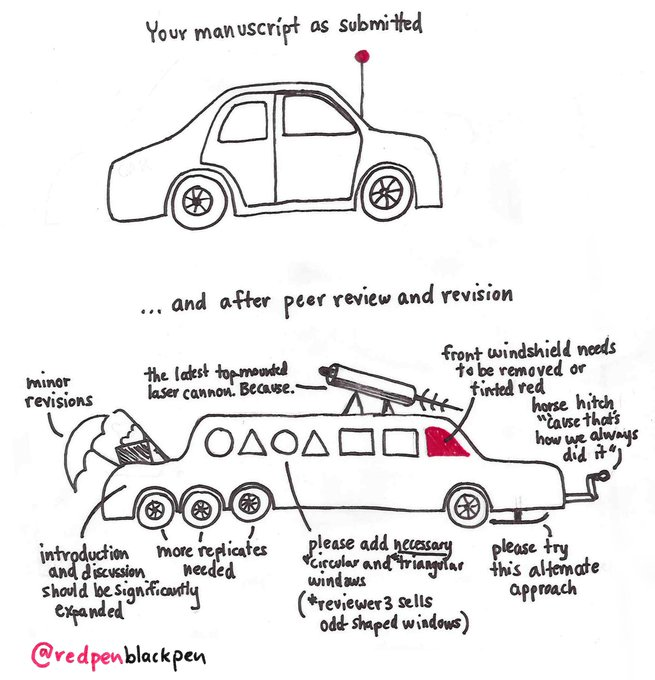
\includegraphics[width=0.4\textwidth]{review.jpg}}
\onslide<3->{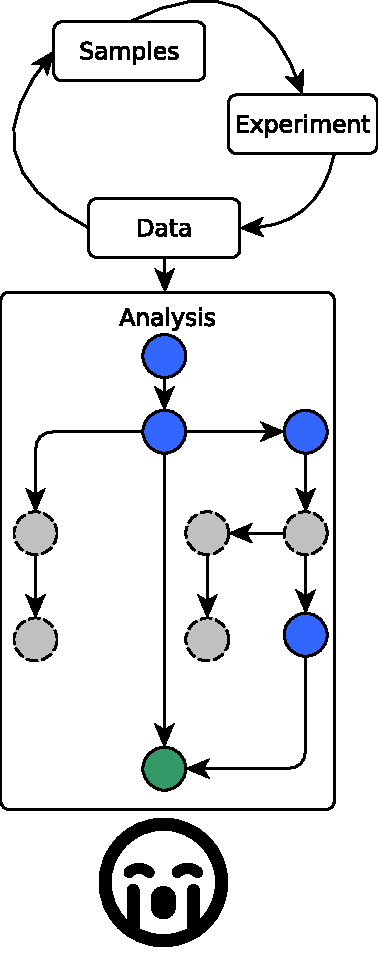
\includegraphics[width=0.17\textwidth]{schema_soumission_fair_echec.pdf}}}
\end{frame}
\begin{frame}{A classic use case}
\centering{What are the changes ?}
\begin{columns}
\column{.5\textwidth}
\begin{itemize}
	\item Tool version
	\item Packages
	\item Environment variables
\end{itemize}
\column{.5\textwidth}
\begin{itemize}
	\item OS version
	\item The computer 
	\item ...
\end{itemize}
\end{columns}
\end{frame}

\begin{frame}
\begin{itemize}
\item Tool compatibility troubles
	\begin{itemize}
	\item Python version ? 2.7, 3.8...
	\item Which tool version ?
	\item Installation without root access
	\item coexistance bewteen severals versions, libraries
	\end{itemize}
\end{itemize}
\end{frame}

\begin{frame}{My python env}
\centering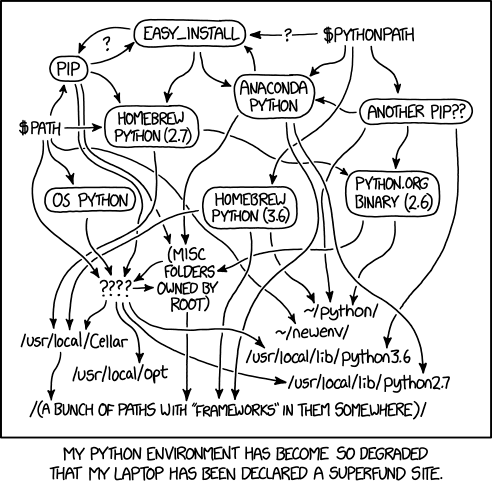
\includegraphics[width=0.5\textwidth]{python_environment.png} 
\end{frame}

\subsection{The use of packaging}
\begin{frame}[<+->]{Encapsulation levels}
\textit{Encapsulation: capture the environment of applications (OS, packages, libraries) to control their execution}
\begin{itemize}[<+->]
	\item Environment management (package manager) 
\includegraphics[width=0.09\textwidth]{conda_logo.pdf} 
	\item Hardware virtualisation (virtual machines) 
\includegraphics[width=0.09\textwidth]{VM_logo.png} 
	\item OS virtualisation (images and containers) 
\includegraphics[width=0.09\textwidth]{docker.pdf} 
\includegraphics[width=0.09\textwidth]{singularity_logo.pdf} 

\end{itemize}
\end{frame}

\subsection{Example with R}
\begin{frame}{Example of R and package installation}{Classical installation}
\begin{itemize}[<+->]
	\item Start with a computer and a specific OS
	\item Inside, we installed a new 
\includegraphics[width=0.3cm, height=0.3cm]{r-project.pdf} application
	\item 
\includegraphics[width=0.3cm, height=0.3cm]{r-project.pdf} need some dependencies
	\item We tested the last  
\includegraphics[width=0.3cm, height=0.3cm]{r-project.pdf} version --> might be conflicts
\end{itemize}

\onslide<1->{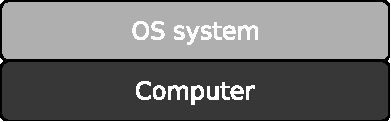
\includegraphics[width=0.25\textwidth]{conda_env_1.pdf}}
\onslide<2->{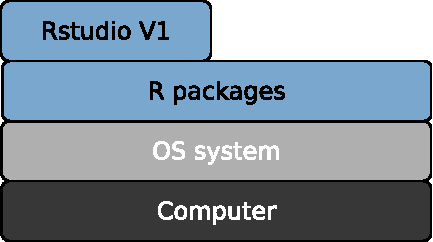
\includegraphics[width=0.25\textwidth]{conda_env_2.pdf}}
\only<3>{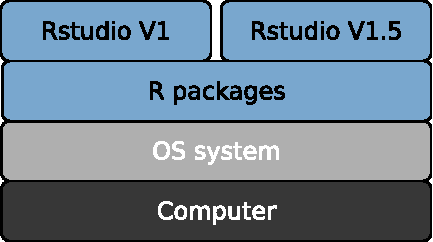
\includegraphics[width=0.25\textwidth]{conda_env_3.pdf}}
\onslide<4->{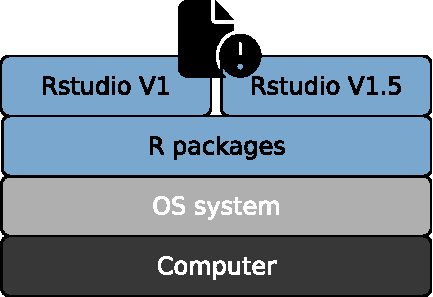
\includegraphics[width=0.25\textwidth]{conda_env_4.pdf}}
\end{frame}

